\documentclass[10pt]{article}
\usepackage[usenames]{color} %used for font color
\usepackage{amssymb} %maths
\usepackage{amsmath} %maths
\usepackage[utf8]{inputenc} %useful to type directly diacritic characters
\usepackage{tikz}
\usetikzlibrary{external}
\usetikzlibrary{quotes,angles}
\usetikzlibrary{decorations.markings}

\begin{document}
\[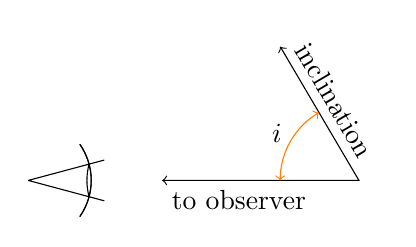
\begin{tikzpicture}
\draw (0,1) -- ++(-15:1) 
          (0,1) -- ++(15:1);
\draw (0,1) ++(35:.8) arc (35:-35:.8);
\draw (0,1) ++(35:.8) arc (35:-35:.8);
\draw (0,1) ++(15:.8) arc (165:195:.8);
\draw
    (1.7, 1) [<->] coordinate (a) node[below right] {to observer}
    -- (4.2,1) coordinate (b) {}
    --  (3.2, 2.7) coordinate (c) node[above right, rotate=-59.534455] {inclination}
    pic["$i$", draw=orange, <->, angle eccentricity=1.2, angle radius=1cm]
    {angle=c--b--a};
\end{tikzpicture}


\]
\end{document}